\documentclass[11pt,a4paper]{article}

\usepackage[T1]{fontenc}
\usepackage{mathpazo}
\usepackage{microtype}
\usepackage[margin=1in]{geometry}
\usepackage{amsmath,amssymb}
\usepackage{booktabs}
\usepackage{graphicx}
\usepackage{xcolor}
\usepackage{tikz}
\usetikzlibrary{arrows.meta,positioning,decorations.pathreplacing}
\usepackage[round,authoryear]{natbib}
\usepackage[font=small,labelfont=bf]{caption}
\usepackage{enumitem}
\usepackage{setspace}
\usepackage{tabularx}
\PassOptionsToPackage{hyphens}{url} % long URLs may break after a hyphen
\usepackage[hidelinks]{hyperref}
\urlstyle{same}

\setstretch{1.12}
\setlist{itemsep=2pt,topsep=4pt}
\newcommand{\tnote}[1]{\par\smallskip{\footnotesize\setstretch{1.0}\noindent\textit{Notes.} #1\par}}
\newcommand{\wide}[1]{\resizebox{\textwidth}{!}{\input{generated/#1}}}

% generated by report/make_report_assets.py -- do not edit
\newcommand{\BkBase}{3.1\%}
\newcommand{\BkFinancePP}{3.0}
\newcommand{\BkFinancet}{8.6}
\newcommand{\BkN}{73{,}295}
\newcommand{\BkOpsPP}{1.5}
\newcommand{\BkOpst}{4.6}
\newcommand{\BreakevenEW}{2.8\%}
\newcommand{\BreakevenOpsVW}{0.6\%}
\newcommand{\BreakevenVW}{1.7\%}
\newcommand{\ConstructCorrHi}{0.97}
\newcommand{\ConstructCorrLo}{0.89}
\newcommand{\CovTwentyTwentyFour}{80\%}
\newcommand{\CovTwoThousandSix}{26\%}
\newcommand{\CovidMean}{\ensuremath{-}19.4\%}
\newcommand{\CushionChangeHi}{2.26}
\newcommand{\CushionChangeLo}{1.70}
\newcommand{\CushionLevelHi}{\ensuremath{-}1.04}
\newcommand{\CushionLevelLo}{\ensuremath{-}2.20}
\newcommand{\DSR}{0.08}
\newcommand{\DSRTrials}{123}
\newcommand{\DSRsrzero}{0.75}
\newcommand{\DevIC}{0.041}
\newcommand{\DevICt}{3.64}
\newcommand{\DevMonths}{96}
\newcommand{\DevNetAlpha}{\ensuremath{-}4.9\%}
\newcommand{\DevNetAlphat}{\ensuremath{-}0.85}
\newcommand{\DevNetMean}{\ensuremath{-}2.1\%}
\newcommand{\DevNetSharpe}{\ensuremath{-}0.12}
\newcommand{\DiagC}{0.0316}
\newcommand{\DiagCM}{0.0423}
\newcommand{\DiagFlag}{0.0351}
\newcommand{\DiagFlagShare}{32\%}
\newcommand{\EvDriftMaxAbst}{1.2}
\newcommand{\EvFirms}{1{,}920}
\newcommand{\EvLegalAbst}{5.1}
\newcommand{\EvMeanAbsCAR}{3.6\%}
\newcommand{\EvN}{15{,}797}
\newcommand{\EvRiskAllCARt}{2.0}
\newcommand{\ExtRiskAllDD}{\ensuremath{-}25\%}
\newcommand{\ExtRiskAllMean}{6.1\%}
\newcommand{\ExtRiskAllSharpe}{0.82}
\newcommand{\ExtRiskAllt}{2.67}
\newcommand{\FMForecastt}{3.32}
\newcommand{\FateBankrupt}{615}
\newcommand{\FateMerged}{2{,}570}
\newcommand{\FateOther}{2{,}846}
\newcommand{\FateSurv}{4{,}139}
\newcommand{\FateTotal}{10{,}170}
\newcommand{\HfourFMmax}{0.89}
\newcommand{\HfourICEnet}{\ensuremath{-}0.0008}
\newcommand{\HfourICLgbm}{0.0001}
\newcommand{\HighRiskSpreadHi}{0.29\%}
\newcommand{\HighRiskSpreadLo}{0.26\%}
\newcommand{\HighRiskSpreadThi}{2.3}
\newcommand{\HighRiskSpreadTlo}{2.1}
\newcommand{\HoneMaxAbsAlphat}{1.97}
\newcommand{\HthreeBest}{$\Delta_{\text{YoY}}$ marketing excellence}
\newcommand{\HthreeMaxT}{2.84}
\newcommand{\HthreeN}{10}
\newcommand{\HtwoMaxAbsT}{1.61}
\newcommand{\HtwoMinT}{\ensuremath{-}1.61}
\newcommand{\HtwoN}{8}
\newcommand{\IncEnet}{0.0090}
\newcommand{\IncEnetAll}{0.0383}
\newcommand{\IncEnetCtrl}{0.0293}
\newcommand{\IncEnetShare}{58\%}
\newcommand{\IncEnett}{1.82}
\newcommand{\IncEns}{0.0066}
\newcommand{\IncEnsAll}{0.0412}
\newcommand{\IncEnsCtrl}{0.0346}
\newcommand{\IncEnsShare}{56\%}
\newcommand{\IncEnst}{1.58}
\newcommand{\IncLgbm}{0.0093}
\newcommand{\IncLgbmAll}{0.0409}
\newcommand{\IncLgbmCtrl}{0.0316}
\newcommand{\IncLgbmShare}{58\%}
\newcommand{\IncLgbmt}{2.05}
\newcommand{\LadderMaxT}{3.9}
\newcommand{\LadderMinT}{2.0}
\newcommand{\LargeIC}{0.028}
\newcommand{\MedianNames}{1{,}118}
\newcommand{\MgBase}{8.3\%}
\newcommand{\MgTecht}{14.3}
\newcommand{\MidIC}{0.026}
\newcommand{\MissHighRisk}{55\%}
\newcommand{\MissLowRisk}{70\%}
\newcommand{\NFeatures}{83}
\newcommand{\NFilings}{131{,}920}
\newcommand{\NFilingsScored}{122{,}600}
\newcommand{\NFirmsPanel}{2{,}247}
\newcommand{\NFirmsScores}{16{,}959}
\newcommand{\NStockMonths}{205{,}574}
\newcommand{\NamesPerLeg}{116}
\newcommand{\OpsCountRho}{\ensuremath{-}0.07}
\newcommand{\OpsFMt}{0.15}
\newcommand{\OpsVWmean}{0.13\%}
\newcommand{\OpsVWt}{0.44}
\newcommand{\OpsWordsRho}{\ensuremath{-}0.38}
\newcommand{\PBO}{0.88}
\newcommand{\PBOsplits}{12{,}870}
\newcommand{\PBOstrategies}{20}
\newcommand{\PaperN}{67{,}727}
\newcommand{\PlaceboDraws}{500}
\newcommand{\PlaceboNullICNinetyFive}{0.0053}
\newcommand{\PlaceboNullNinetyFive}{0.64}
\newcommand{\PlaceboPic}{0.000}
\newcommand{\PlaceboPsharpe}{0.042}
\newcommand{\PlaceboRealSharpe}{0.70}
\newcommand{\RepFirms}{5{,}832}
\newcommand{\RepInter}{0.149}
\newcommand{\RepIntert}{0.37}
\newcommand{\RepN}{34{,}960}
\newcommand{\RepOpFour}{0.289}
\newcommand{\RepOpFourSE}{0.107}
\newcommand{\RepOpFourt}{2.69}
\newcommand{\RepOpTwo}{0.275}
\newcommand{\RepOpTwoSE}{0.100}
\newcommand{\RepSize}{0.415}
\newcommand{\RepYearHi}{2024}
\newcommand{\RepYearLo}{2008}
\newcommand{\RiskAllEWalphat}{1.95}
\newcommand{\RiskAllEWmean}{0.43\%}
\newcommand{\RiskAllEWt}{2.65}
\newcommand{\RiskAllFMcoef}{0.83\%}
\newcommand{\RiskAllFMt}{2.61}
\newcommand{\RiskAllVWalphat}{1.45}
\newcommand{\RiskAllVWmean}{0.26\%}
\newcommand{\RiskAllVWt}{2.15}
\newcommand{\ShapCtrl}{37\%}
\newcommand{\ShapInter}{3\%}
\newcommand{\ShapLeaves}{15}
\newcommand{\ShapMkt}{43\%}
\newcommand{\ShapRisk}{17\%}
\newcommand{\ShapTop}{r\_rev\_1}
\newcommand{\ShapTrees}{90}
\newcommand{\ShuffledIC}{0.0073}
\newcommand{\ShuffledICt}{1.37}
\newcommand{\SingleSortCount}{42}
\newcommand{\SingleSortMaxAbsAlphat}{2.84}
\newcommand{\SmallIC}{0.051}
\newcommand{\SmallLSt}{3.02}
\newcommand{\SmallSharpe}{0.97}
\newcommand{\SpecCount}{123}
\newcommand{\SubAt}{\ensuremath{-}0.72}
\newcommand{\SubBt}{\ensuremath{-}0.58}
\newcommand{\TestEnd}{2025-05}
\newcommand{\TestGrossSharpe}{0.80}
\newcommand{\TestIC}{0.060}
\newcommand{\TestICControls}{0.064}
\newcommand{\TestICt}{4.52}
\newcommand{\TestMonths}{41}
\newcommand{\TestNetAlpha}{\ensuremath{-}4.6\%}
\newcommand{\TestNetAlphat}{\ensuremath{-}0.83}
\newcommand{\TestNetMean}{8.9\%}
\newcommand{\TestNetMeant}{1.46}
\newcommand{\TestNetSharpe}{0.51}
\newcommand{\TestStart}{2022-01}
\newcommand{\Turnover}{214\%}
\newcommand{\TurnoverOneWay}{54\%}
\newcommand{\VolAccountingt}{\ensuremath{-}11.7}
\newcommand{\VolAllt}{\ensuremath{-}1.04}
\newcommand{\VolDown}{3}
\newcommand{\VolFinancet}{\ensuremath{-}3.8}
\newcommand{\VolInternationalt}{0.4}
\newcommand{\VolLegalt}{6.0}
\newcommand{\VolManagementt}{\ensuremath{-}5.7}
\newcommand{\VolMarketingt}{3.4}
\newcommand{\VolOperationst}{0.1}
\newcommand{\VolOpst}{0.10}
\newcommand{\VolSigCount}{5}
\newcommand{\VolTechnologyt}{2.9}
\newcommand{\VolUp}{2}


\title{\textbf{Reading the Risk Factors}\\[4pt]
\large Do 10-K Risk Disclosures and Earnings-Call Marketing Language\\ Predict U.S. Stock Returns?}
\author{Yug Mitulkumar Desai \qquad Arin Mehta\\[8pt]
{\normalsize Supervisor: Professor Marcos Severo}\\[2pt]
{\normalsize MS 499 Independent Research}}
\date{November 2026}

\begin{document}
\maketitle

\begin{abstract}
\noindent
We test whether two recently published text datasets carry information about U.S. stock returns that is not already in
standard firm characteristics. The first is the transformer-based scores of Astvansh and Simpson (2026), which measure
how much the risk-factor section (Item 1A) of each 10-K discusses eight types of risk. The second is the sentence-embedding
scores of Damavandi, Mai and Astvansh (2025), which measure how much managers emphasise marketing in earnings calls.
We build a strictly point-in-time monthly panel of \NFirmsPanel{} firms and \NStockMonths{} stock-months (2010--2025)
from free data, pre-register five hypotheses, and evaluate them with portfolio sorts, Fama-MacBeth regressions and a
walk-forward machine-learning ladder. The final \TestMonths{} months were locked until the design was frozen.
The forecasts rank stocks better than chance: the mean monthly rank information coefficient of the ensemble is
\DevIC{} ($t=\DevICt$) in 2014--2021 and \TestIC{} ($t=\TestICt$) in the locked test. But a controls-only model does as well
(\TestICControls{} in the test), the long-short strategy earns no significant alpha after the Fama-French five factors,
momentum and 25 basis points of trading costs ($t=\DevNetAlphat$ and $\TestNetAlphat$), and multiple-testing diagnostics
(deflated Sharpe probability \DSR{} over \DSRTrials{} trials; probability of backtest overfitting \PBO) confirm that no
specification is a reliable strategy. The text is informative about risk rather than about expected returns:
individual risk categories predict future volatility, finance-risk language predicts bankruptcy within three years,
legal-risk language predicts larger filing-day price moves, and the source paper's main operational result replicates
on independent accounting data. A survivorship audit using SEC filing histories shows that the free-data bias works
against, not for, the small risk premium we observe.
\end{abstract}

\vspace{4pt}
\noindent\textbf{Keywords:} textual analysis; risk-factor disclosure; earnings calls; marketing; cross-section of returns;
machine learning; backtest overfitting.

\vspace{6pt}
{\small\noindent\begin{tabularx}{\linewidth}{@{}l>{\raggedright\arraybackslash}X@{}}
\textbf{Code and data:} & \url{https://github.com/Yugdes/Long-Short-Equity-Strategy-from-10-K-Earnings-Call-NLP-Signals}\\
\textbf{Website:} & \url{https://yugdes.github.io/Long-Short-Equity-Strategy-from-10-K-Earnings-Call-NLP-Signals/}
\end{tabularx}}

\newpage
\tableofcontents
\newpage

%=====================================================================
\section{Introduction}
%=====================================================================

Every U.S. public company must describe, in Item 1A of its annual 10-K, the risks that could hurt its business. Every quarter,
its managers also explain their results to analysts in an earnings call. Both are long, mostly unstructured texts, and both
are read by investors. A growing literature shows that the language of such documents can move prices and, sometimes,
predict them \citep{loughran2011,price2012,cohen2020}. Two recent papers turned these texts into ready-made firm-level
measures. \citet{astvansh2026} fine-tuned transformer classifiers to score how strongly each 10-K risk section discusses
eight types of risk (accounting, finance, international, legal, management, marketing, operations and technology) for
\NFilings{} firm-years. \citet{damavandi2025} used sentence embeddings to score how much managers emphasise market
orientation, marketing capabilities and marketing excellence in earnings calls. Neither paper asks whether the measures
predict stock returns.

This study asks exactly that. Our question is narrow and practical: \emph{once everything an investor could have known
at the time is used correctly, do these text scores help predict next month's cross-section of returns, beyond the
characteristics that are already known to do so, and does that help survive trading costs and standard factor
adjustments?} We also ask a related question on which the economics are clearer: do the risk scores tell investors
something about \emph{risk}, such as future volatility, distress or the market's reaction when a filing appears?

We take three precautions that much of the backtesting literature does not.
\begin{enumerate}
  \item \textbf{Point in time.} Every input enters the panel only after it was public, plus a lag: a 10-K score from the
  first full month after the filing date plus two business days, a call score from two months after its calendar quarter
  ends, and accounting and price controls from the end of the previous month. Unit tests check these rules on the final panel.
  \item \textbf{Pre-registration and a locked test window.} The hypotheses, the primary strategy and the significance
  hurdle were written down before any return was examined. The last \TestMonths{} months (\TestStart{} to \TestEnd) were locked by
  code until the design was frozen, then run once.
  \item \textbf{Honest accounting for search.} Every development-window specification is logged, and the primary
  strategy is judged with a deflated Sharpe ratio \citep{bailey2014} over that log, the probability of backtest
  overfitting \citep{bailey2017}, a $|t|\geq 3$ hurdle \citep{hlz2016}, placebo shuffles and a shuffled-label retraining.
\end{enumerate}

\paragraph{Findings.} The answer to the return question is negative. The machine-learning forecasts rank stocks better
than chance in both windows (rank IC \DevIC{} and \TestIC), but a model that uses only ten standard characteristics ranks
them as well, and the value-weighted decile long-short portfolio earns no significant alpha net of costs. None of the
pre-registered return hypotheses clears the hurdle. Higher disclosed risk is, if anything, associated with slightly
\emph{higher} subsequent returns, consistent with a risk premium rather than mispricing, but the effect is not robust.
The answer to the risk question is more positive. Individual risk categories predict next-year return volatility
(\VolSigCount{} of 8 with $|t|\geq3$ after controls, in both directions). Finance-risk language predicts bankruptcy within
three years ($t=\BkFinancet$). Legal-risk language predicts larger price moves on the filing day ($t=\EvLegalAbst$).
The source paper's link between operational risk and next-year cost of goods sold replicates on SEC XBRL data
(coefficient \RepOpFour{} against their 0.247). The scores therefore measure something real about firms; that
information is simply not a source of abnormal returns.

\paragraph{Contributions.} (i) We provide the first out-of-sample return test of both datasets under strict point-in-time
rules. (ii) We document data issues a user of these datasets must handle, notably that the risk data's fiscal-year field
is the filing year. (iii) We show how free data can be audited for survivorship bias with SEC filing histories, and that
in this setting the bias works against the risk premium. (iv) We report a look-ahead bug that our locked test window
exposed (Appendix~\ref{app:bug}), as a cautionary example of how free price data can leak the future.

\paragraph{Roadmap.} Section~\ref{sec:lit} reviews the literature. Section~\ref{sec:data} describes the data and
Section~\ref{sec:design} the research design. Section~\ref{sec:results} reports the hypothesis tests and the strategy,
Section~\ref{sec:robust} the robustness and overfitting checks, and Section~\ref{sec:further} three supplementary studies.
Section~\ref{sec:discussion} discusses, Section~\ref{sec:limits} lists limitations and Section~\ref{sec:conclusion} concludes.

%=====================================================================
\section{Related literature}\label{sec:lit}
%=====================================================================

\paragraph{Text in finance.} \citet{loughran2011} show that general-purpose sentiment dictionaries misclassify financial
language and build finance-specific word lists that relate to filing-period returns, volume and volatility.
\citet{cohen2020} find that firms that change the language of their 10-Ks underperform: a portfolio short ``changers''
earns large alphas with no announcement effect, which they attribute to investor inattention. Their result motivates our
test of risk \emph{changes} (H2) and our skipping of the filing month.

\paragraph{Risk-factor disclosure.} Item 1A became mandatory for 10-Ks filed after 1 December 2005.
\citet{campbell2014} show that firms facing more risk disclose more, that the type of risk shapes the type of disclosure,
and that disclosure is reflected in systematic and idiosyncratic risk and in firm value. \citet{kravet2013} find that
increases in risk disclosure raise return volatility and trading volume around and after the filing. Both papers
suggest that risk disclosure is informative about \emph{risk}; whether it predicts \emph{returns} depends on whether that
risk is priced or mispriced. \citet{astvansh2026}, the source of our risk scores, link operational risk to higher
operational cost in the following year and make no return claims. Their eight risk types, keyword dictionaries and
Item 1A extraction follow \citet{schnatterly2021}, who classify each firm's risk-factor headings into the same eight domains
as the expertise of its directors. Firms whose boards lack expertise in the domains of their disclosed risks earn lower
abnormal stock returns over the next fiscal year (S\&P 1500 firms, 2006--2017). In that study, risk disclosure is linked to
returns through governance, not directly.

\paragraph{Earnings calls and marketing.} \citet{price2012} show that the tone of earnings calls predicts abnormal returns
beyond the earnings surprise, with part of the response delayed over about a quarter. The marketing-finance literature
argues that marketing assets create firm value that investors may price slowly \citep{srinivasan2009}; a meta-analysis
finds elasticities of firm value of about 0.04 for advertising spending and 0.54 for marketing assets
\citep{edeling2016}. \citet{damavandi2025} validate their marketing-emphasis scores against advertising intensity but do
not test returns.

\paragraph{Machine learning and replication.} \citet{gkx2020} show that tree ensembles and neural networks improve
return forecasts, mainly through momentum, liquidity and volatility signals, with monthly out-of-sample $R^2$ well below
1\%. Our model menu and walk-forward design follow theirs. A large literature warns that most published anomalies are
weaker than reported: \citet{hlz2016} argue for $t$-statistics of at least 3, \citet{mclean2016} find that anomaly returns
fall by about a third after publication, and \citet{jkp2023} show that capped value weights and factor adjustment matter
for replication. The deflated Sharpe ratio of \citet{bailey2014} and the probability of backtest overfitting of
\citet{bailey2017} account for specification search, and we apply both to our own.

%=====================================================================
\section{Data}\label{sec:data}
%=====================================================================

\subsection{Text scores}

\paragraph{Risk scores.} The \citet{astvansh2026} release covers \NFilings{} 10-K filings by \NFirmsScores{} firms (CIKs),
filed from January 2005 to January 2025. For each filing it reports, for each of the eight risk types of
\citet{schnatterly2021} (accounting, finance, international, legal, management, marketing, operations and technology), a
count from that paper's keyword dictionaries
and a transformer probability that the risk section ``mentions'' that type, together with the section's word count and a
flag for firms for which Item 1A was optional. The transformers were fine-tuned on 761 synthetic sentences generated by a
language model and labelled by dictionary presence; the best of eight architectures was kept for each type (mostly
BERT-base; \citealp{devlin2019}). Our audit of the data (Appendix~\ref{app:audit}) found three issues that matter for a
return study:
\begin{enumerate}
  \item The \texttt{FYEAR} field equals the calendar year of the filing date in 100\% of rows; it is not the Compustat fiscal
  year. We key every timing rule on the filing date, which matches an original 10-K in EDGAR for all but three rows.
  \item Filings from 2005 almost never contain an Item 1A section (the mandate began in December 2005), and
  sections with zero words carry probabilities of exactly zero. We treat them as missing, which leaves \NFilingsScored{}
  scored sections.
  \item The probabilities track their own dictionary counts only loosely: among sections of at least 1,000 words, the
  operations probability's rank correlation with its dictionary count is \OpsCountRho, and with section length
  \OpsWordsRho. The probability behaves like the \emph{share} of the section devoted to a risk type, not its amount.
\end{enumerate}
Figure~\ref{fig:scores} shows the mean probabilities and the median length of Item 1A over time. Sections roughly
quadrupled in length between 2006 and 2024, so we only ever compare scores within a cross-section.

\begin{figure}[tbp]
\centering
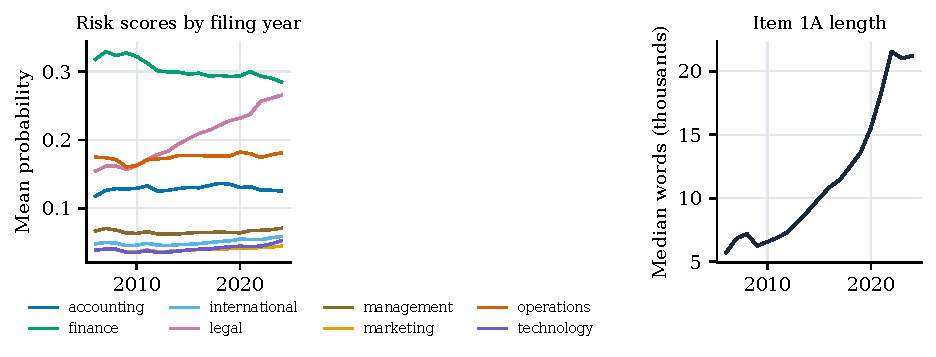
\includegraphics[width=\textwidth]{figures/scores.pdf}
\caption{Risk scores and Item 1A length by filing year. Left: mean transformer probability of each risk type. Right:
median number of words in Item 1A among non-empty sections.}
\label{fig:scores}
\end{figure}

\paragraph{Marketing-emphasis scores.} The \citet{damavandi2025} executive file (version 2) covers 337,599 firm-quarters
of earnings calls for 11,296 Compustat firms (GVKEYs) from 2003 to 2025. Each call paragraph is embedded with SBERT
\citep{reimers2019}, and each of 19 marketing components is scored by cosine similarity to the centroid of its
dictionary terms, averaged over the call. The components group into market orientation (8 components), marketing
capabilities (8) and marketing excellence (3); the authors also supply ZCA-whitened versions to reduce anisotropy. The
three constructs are nearly collinear in our sample (pairwise correlations \ConstructCorrLo{} to \ConstructCorrHi), so the
whitened components carry most of the distinct information. We verified on seven IPO firms with known first calls that the
\texttt{quarter} field is the calendar quarter of the call. Scores are linked from GVKEY to CIK with the WRDS SEC linking
table, using only links valid at the end of the quarter and discarding ambiguous matches.

\subsection{Market and accounting data}

No CRSP or Compustat return files were available, so the study uses free sources, frozen after download:
\begin{itemize}
  \item \textbf{Prices}: Yahoo Finance daily bars with dividends and splits for every current SEC ticker, aggregated to monthly
  total returns. Impossible returns (below $-100\%$ or above $+1{,}000\%$) are removed.
  \item \textbf{Shares outstanding and fundamentals}: SEC XBRL company facts \citep{secedgar}, which record the date each value
  was filed, so they are point in time. XBRL begins in 2009--2011, which is why the primary sample starts in 2010.
  Market capitalisation is the split-adjusted price times split-adjusted shares, with sanity rules for misreported share
  counts (Appendix~\ref{app:decisions}).
  \item \textbf{Industries}: current SIC codes from SEC submissions, mapped to the Fama-French 12 and 48 industries.
  \item \textbf{Factors}: Fama-French five factors, momentum and the risk-free rate from Kenneth French's data library
  \citep{frenchlib}; daily factors for the event study.
\end{itemize}
We checked the free data against known benchmarks. Our momentum and size long-short returns correlate 0.83 and 0.84
with the published UMD and SMB factors, and market capitalisations match public values for large firms (for example,
NVIDIA at about \$2.7 trillion in May 2024).

\subsection{Universe and coverage}

The primary universe in month $t$ contains common stocks with a price of at least \$5 and a market capitalisation of at
least \$100 million at the end of $t-1$, at least twelve months of return history, a live risk signal, and a non-financial,
non-utility SIC code. It contains \NFirmsPanel{} firms and \NStockMonths{} stock-months from 2010-01 to 2025-05, with a
median of \MedianNames{} stocks per month. The sample ends in 2025-05 because the risk data stop with filings made in
early 2025: in 2025-06 the 15-month staleness cap expires the February 2024 filers and the universe halves.
Table~\ref{tab:funnel} shows how each year's 10-K filings reach the universe. Most attrition comes from firms without a
current ticker, which include registrants that never had listed equity and firms that have since disappeared.
Section~\ref{sec:surv} audits the second group.

\begin{table}[tbp]
\centering
\caption{From 10-K filings to the primary universe}
\label{tab:funnel}
\wide{tab_funnel}
\tnote{Counts of risk-dataset filings by filing year. ``Current SEC ticker'': the filer has a ticker in today's SEC
ticker file; ``Yahoo prices'': prices were returned; ``Extended universe'': equal-weighted sample from 2006 without size
data; ``Primary universe'': passes all screens in at least one month.}
\end{table}

%=====================================================================
\section{Research design}\label{sec:design}
%=====================================================================

\subsection{Timing rules}

Figure~\ref{fig:timing} summarises when each input becomes usable. A 10-K filed on date $d$ is first used in the first
full calendar month after $d$ plus two business days, and is dropped 15 months after its filing month if no newer filing
arrives. A call score for calendar quarter $q$ is first used in the second month after $q$ ends (one month of buffer on
top of the quarter end, since call dates are not supplied) and expires after six months. Price-based controls are measured
at the end of month $t-1$; accounting values become usable one month after the month in which they were filed. All
cross-sectional transformations (ranks, imputation, the value-weight cap) use only the current month's eligible stocks.
Unit tests assert, on the final panel, that no signal is used before its release and that no signal outlives its cap.

\begin{figure}[tbp]
\centering
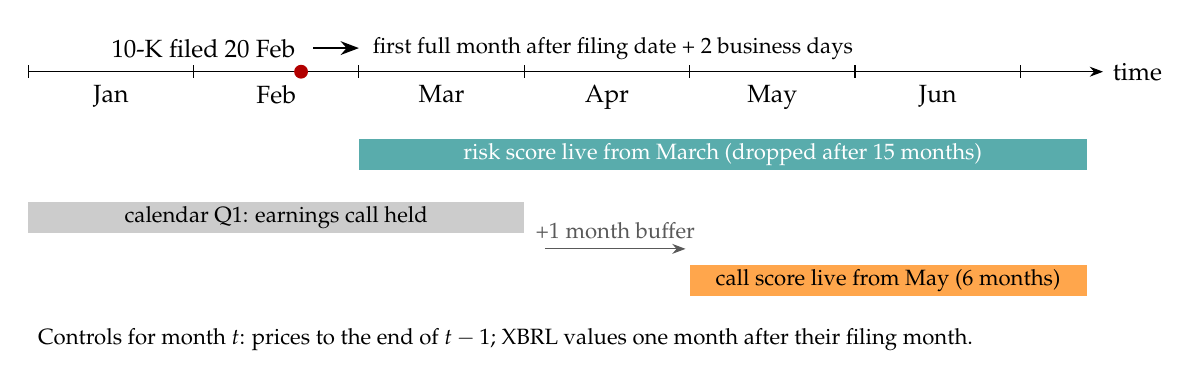
\begin{tikzpicture}[x=1.05cm,y=1cm,font=\small]
  \draw[-{Stealth}] (0,0) -- (13,0) node[right] {time};
  \foreach \i in {0,2,...,12} { \draw (\i,0.08) -- (\i,-0.08); }
  \foreach \i/\l in {1/Jan,3/Feb,5/Mar,7/Apr,9/May,11/Jun} { \node[below] at (\i,-0.05) {\l}; }
  \fill[red!70!black] (3.3,0) circle (2.5pt);
  \node[above left] at (3.35,0.05) {10-K filed 20 Feb};
  \draw[-{Stealth},thick] (3.45,0.3) -- (4,0.3);
  \node[right,align=left] at (4.05,0.3) {\footnotesize first full month after filing date + 2 business days};
  \fill[teal!65] (4,-0.85) rectangle (12.8,-1.25);
  \node[white] at (8.4,-1.05) {\footnotesize risk score live from March (dropped after 15 months)};
  \fill[gray!40] (0,-1.65) rectangle (6,-2.05);
  \node at (3,-1.85) {\footnotesize calendar Q1: earnings call held};
  \draw[-{Stealth},gray!70!black] (6.25,-2.25) -- (7.95,-2.25) node[midway,above] {\footnotesize +1 month buffer};
  \fill[orange!70] (8,-2.45) rectangle (12.8,-2.85);
  \node at (10.4,-2.65) {\footnotesize call score live from May (6 months)};
  \node[anchor=west] at (0,-3.4) {\footnotesize Controls for month $t$: prices to the end of $t-1$; XBRL values one month after their filing month.};
\end{tikzpicture}
\caption{Point-in-time rules. A 10-K filed on 20 February is first used in March's portfolio; a call held in the first
calendar quarter is first used in May's.}
\label{fig:timing}
\end{figure}

\subsection{Features and target}

Every feature is a centred cross-sectional percentile rank in $[-0.5,0.5]$, computed each month over eligible stocks; a
missing value is set to 0, the month's median. There are \NFeatures{} features in four groups:
\begin{itemize}
  \item \textbf{Controls (10)}: log market capitalisation, log book-to-market, momentum from $t-12$ to $t-2$
  \citep{jegadeesh1993}, one-month reversal \citep{jegadeesh1990}, 12-month volatility \citep{ang2006}, 36-month CAPM beta,
  Amihud illiquidity \citep{amihud2002}, log dollar volume, asset growth \citep{cooper2008} and gross profitability
  \citep{novymarx2013}.
  \item \textbf{Risk text (36)}: the eight probabilities, the mean of the seven non-operational probabilities, the operations
  count density and log section length; for each, the change against the firm's previous 10-K (within 18 months) and the
  surprise against the firm's own history (expanding mean of at least two prior filings); plus an aggregate risk rank
  (the mean rank of the eight probabilities), its change, and industry-demeaned operations risk.
  \item \textbf{Marketing (30)}: the three constructs, the 19 whitened components, analysts' customer orientation,
  quarter-on-quarter and year-on-year changes of the constructs, and a flag for call coverage.
  \item \textbf{Interactions (7)}: operations $\times$ non-operational risk, and operations risk (level and change)
  $\times$ each marketing construct.
\end{itemize}
The machine-learning target is the centred rank of the month-$t$ excess return; a three-month cumulative return is used
as a robustness target.

\subsection{Hypotheses}

Table~\ref{tab:hyp} lists the five hypotheses and their deciding tests, as written before any return was examined. The
literature does not fix every sign. Disclosure levels that load on systematic risk \citep{campbell2014} predict a risk
premium (H1); the inattention story of \citet{cohen2020} predicts that rising risk language precedes underperformance (H2);
the marketing literature predicts that marketing emphasis signals intangible value that is priced slowly (H3).

\begin{table}[tbp]
\centering
\caption{Pre-registered hypotheses}
\label{tab:hyp}
\small
\begin{tabularx}{\textwidth}{@{}lXX@{}}
\toprule
 & Hypothesis and predicted sign & Deciding test (development window) \\
\midrule
H1 & Risk \emph{levels} are priced as risk, not mispricing: operations and aggregate risk predict higher future volatility, and their long-short portfolios earn no alpha. & Fama-MacBeth of next-12-month volatility on the risk rank with controls; decile long-short FF5 + momentum alpha. \\
H2 & Firms whose disclosed risk \emph{rises} underperform (negative). & Decile long-short and Fama-MacBeth on the change in operations and aggregate risk. \\
H3 & Marketing emphasis predicts higher returns (positive). & Decile long-short and Fama-MacBeth on construct levels and year-on-year changes, marketing-covered stocks. \\
H4 & Marketing emphasis softens the return penalty of high or rising operational risk (interaction positive). & 3$\times$3 conditional double sorts; Fama-MacBeth with the interaction; incremental IC of interaction features. \\
H5 & A machine-learning model on text and controls beats controls alone and survives costs. & Paired monthly IC difference; primary strategy net-of-cost FF5 + momentum alpha. \\
\bottomrule
\end{tabularx}
\tnote{The significance hurdle for every headline test is $|t|\geq 3$ in the predicted direction \citep{hlz2016}.
$t$-statistics use Newey-West standard errors with six lags \citep{neweywest1987}.}
\end{table}

\subsection{Evaluation framework}

\paragraph{Portfolio sorts and regressions.} Single-signal tests use monthly decile portfolios (top minus bottom),
equal-weighted and value-weighted. Value weights use market capitalisation capped at the 80th percentile of NYSE-listed
stocks in the universe each month, following \citet{jkp2023}, which prevents a few mega-caps from dominating a leg.
Alphas come from time-series regressions on the CAPM, FF3 \citep{ff1993}, FF5 \citep{ff2015}, FF5 plus momentum
\citep{carhart1997}, and FF5 plus momentum plus a low-volatility factor built inside our own universe
\citep{frazzini2014}. Fama-MacBeth regressions \citep{famamacbeth1973} use the ranks of the signal and the ten controls.

\paragraph{Walk-forward machine learning.} Four learners (elastic net, \citealp{zou2005}; LightGBM, \citealp{ke2017};
XGBoost, \citealp{chen2016}; and a two-layer neural network) are trained on an expanding window and refit every January
for each test year from 2014. Hyperparameters are tuned on the last two years of each training window. The month before
each test year is left out of training as an embargo \citep{lopezdeprado2018}, so training labels end in November, and
the fitting and validation slices are separated by the same one-month gap (longer for the three-month target). The ensemble averages the four learners' within-month prediction ranks. The
feature sets form a ladder (controls; plus risk; plus marketing; plus interactions), always estimated on identical rows,
so that differences measure what each block adds.

\paragraph{Primary strategy.} Fixed in advance: the ensemble forecast from all features, value-weighted top-minus-bottom
decile, rebalanced monthly, net of 25 basis points one-way on every dollar traded. Turnover accounts for weight drift.
Equal-weighted, quintile and sector-neutral versions are secondary.

\paragraph{Multiple testing.} Every portfolio or model specification evaluated on the development window is appended to a
log; \SpecCount{} were logged in total. The deflated Sharpe ratio uses the dispersion of their Sharpe ratios as the null.
The probability of backtest overfitting uses combinatorially symmetric cross-validation over 16 blocks. A placebo test
re-runs the primary portfolio \PlaceboDraws{} times with forecasts shuffled within each month, and a shuffled-label test
retrains LightGBM on targets shuffled within each month.

\paragraph{Windows.} Development: 2010--2021 for sorts and regressions, 2014--2021 (\DevMonths{} months) for
out-of-sample forecasts. Locked test: \TestStart{} to \TestEnd{} (\TestMonths{} months), unlocked once after the
design was frozen.

%=====================================================================
\section{Results}\label{sec:results}
%=====================================================================

\subsection{Single signals: H1, H2 and H3}

Table~\ref{tab:single} reports each pre-registered signal and the exploratory individual risk factors. None of the
\SingleSortCount{} portfolio tests clears the $|t|\geq3$ hurdle; the largest factor-adjusted alpha has $|t|=\SingleSortMaxAbsAlphat$.

\textbf{H1 (risk levels).} Operations risk carries no return premium: its value-weighted decile spread is \OpsVWmean{} a
month ($t=\OpsVWt$) and its Fama-MacBeth slope with controls has $t=\OpsFMt$. The aggregate risk rank does better: firms with
the most risk language earn \RiskAllVWmean{} a month more than those with the least (value-weighted, $t=\RiskAllVWt$;
equal-weighted \RiskAllEWmean, $t=\RiskAllEWt$), and the Fama-MacBeth slope with controls has $t=\RiskAllFMt$. The sign is
that of a risk premium, as H1 predicts, but the effect falls below the hurdle and largely disappears after factor
adjustment ($t_\alpha=\RiskAllVWalphat$). The no-alpha half of H1 therefore holds (largest $|t_\alpha|$ among level sorts
\HoneMaxAbsAlphat). The volatility half is in Section~\ref{sec:vol}.

\textbf{H2 (risk changes).} Rising risk language does not predict lower returns. Across \HtwoN{} statistics on changes and
surprises, the most negative is $t=\HtwoMinT$. Unlike the 10-K language changes of \citet{cohen2020}, changes in these
probabilities carry no return information.

\textbf{H3 (marketing).} All marketing statistics have the predicted positive sign, and Fama-MacBeth slopes with
controls reach $t\approx2$ for all three constructs, but the best of \HthreeN{} statistics (\HthreeBest) has $t=\HthreeMaxT$,
below the hurdle.

\begin{table}[tbp]
\centering
\caption{Single-signal tests, development window 2010--2021}
\label{tab:single}
\wide{tab_single}
\tnote{Value-weighted (capped) decile long-short portfolios, top minus bottom; $\alpha$ from FF5 + momentum; EW $t_\alpha$ is
the equal-weighted version. FM slope: Fama-MacBeth coefficient on the centred rank (so the slope is the predicted return
difference between the lowest- and highest-ranked stock, in \% per month), with ten controls. Marketing signals use
marketing-covered stocks only. Bold: $|t|\geq3$. Newey-West(6) $t$-statistics.}
\end{table}

\subsection{Risk language and future volatility}\label{sec:vol}

The pre-registered volatility test of H1 fails. Neither operations risk ($t=\VolOpst$) nor the aggregate risk rank
($t=\VolAllt$) predicts higher next-12-month volatility once the controls, which include past volatility, are in the
regression (Table~\ref{tab:vol}). The individual factors tell a different story (Figure~\ref{fig:vol}). Legal ($t=\VolLegalt$)
and marketing risk ($t=\VolMarketingt$) predict \emph{higher} volatility; accounting ($t=\VolAccountingt$), management
($t=\VolManagementt$) and finance risk ($t=\VolFinancet$) predict \emph{lower} volatility. Because the effects have opposite
signs, they cancel in the aggregate. A plausible reading, consistent with the share interpretation of the probabilities,
is that mature, stable firms devote their risk sections to accounting and financing boilerplate, while firms facing
litigation or fast-changing markets devote theirs to legal and market risks. These results were found by exploring the
eight factors, not predicted, and should be read as such.

\begin{figure}[tbp]
\centering
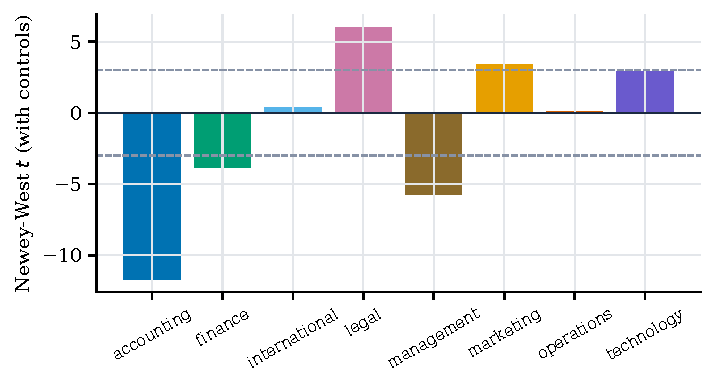
\includegraphics[width=0.78\textwidth]{figures/vol.pdf}
\caption{Do individual risk factors predict next-year volatility? Newey-West $t$-statistics of Fama-MacBeth slopes of the
next-12-month volatility rank on each risk factor's rank, with the ten controls (including past volatility). Dashed lines:
$\pm3$.}
\label{fig:vol}
\end{figure}

\begin{table}[tbp]
\centering
\caption{Risk language and next-12-month volatility, 2010--2020}
\label{tab:vol}
\small
\begin{tabular}{lrrrr}
\toprule
Signal & Slope alone & $t$ & Slope with controls & $t$ \\
\midrule
\multicolumn{5}{l}{\textit{Pre-registered (H1a)}} \\
Operations risk & 0.018 & 1.08 & 0.001 & 0.10 \\
Aggregate risk (8 factors) & \ensuremath{-}0.028 & \ensuremath{-}1.38 & \ensuremath{-}0.008 & \ensuremath{-}1.04 \\
Non-operational risk (7 factors) & \ensuremath{-}0.091 & \textbf{\ensuremath{-}9.84} & \ensuremath{-}0.023 & \textbf{\ensuremath{-}7.45} \\
Operations risk, industry-demeaned & 0.081 & \textbf{16.79} & 0.011 & 2.38 \\
Operations count density & 0.017 & 1.00 & \ensuremath{-}0.001 & \ensuremath{-}0.11 \\
\midrule
\multicolumn{5}{l}{\textit{Exploratory: individual factors}} \\
Accounting risk & \ensuremath{-}0.121 & \textbf{\ensuremath{-}18.21} & \ensuremath{-}0.043 & \textbf{\ensuremath{-}11.69} \\
Finance risk & \ensuremath{-}0.116 & \textbf{\ensuremath{-}6.27} & \ensuremath{-}0.030 & \textbf{\ensuremath{-}3.82} \\
International risk & \ensuremath{-}0.072 & \textbf{\ensuremath{-}4.81} & 0.002 & 0.38 \\
Legal risk & 0.097 & \textbf{6.25} & 0.037 & \textbf{6.01} \\
Management risk & \ensuremath{-}0.038 & \textbf{\ensuremath{-}6.52} & \ensuremath{-}0.026 & \textbf{\ensuremath{-}5.73} \\
Marketing risk & 0.104 & \textbf{6.14} & 0.028 & \textbf{3.37} \\
Technology risk & 0.096 & \textbf{11.27} & 0.024 & 2.92 \\
\bottomrule
\end{tabular}

\tnote{Fama-MacBeth regressions of the cross-sectional rank of realised volatility over months $t$ to $t+11$ on the
signal's rank, alone and with the ten controls. Formation months end in 2020-12 so that the forward window never reaches the
locked test period. Bold: $|t|\geq3$.}
\end{table}

\subsection{Does marketing cushion operational risk? H4}

H4 predicts that marketing emphasis softens the return penalty of high or rising operational risk. We test it three ways.
First, the Fama-MacBeth interaction slopes are positive in most specifications but never significant (largest
$t=\HfourFMmax$; Table~\ref{tab:hfourfm}). Second, adding the interaction features to the model changes its IC by
\HfourICEnet{} (elastic net) and \HfourICLgbm{} (LightGBM). Third, the pre-registered $3\times3$ conditional double sort
splits stocks into thirds by operations risk and then into thirds by marketing within each risk third
(Table~\ref{tab:hfourds}). The ``cushion'' is how much more high-marketing firms beat low-marketing firms among the riskiest
third than among the safest. For the risk \emph{level} it has the wrong sign (value-weighted $t_\alpha$ from \CushionLevelLo{}
to \CushionLevelHi). For the risk \emph{change} it has the predicted sign in all three constructs ($t_\alpha$ \CushionChangeLo{}
to \CushionChangeHi): among firms whose operational risk rose most, high-marketing firms earned \HighRiskSpreadLo{} to
\HighRiskSpreadHi{} a month more than low-marketing firms ($t_\alpha$ \HighRiskSpreadTlo{} to \HighRiskSpreadThi). None of this
clears the hurdle, and since rising risk carries no return penalty of its own (H2), there is little to cushion. We
classify H4 as below the hurdle.

\begin{table}[tbp]
\centering
\caption{H4: risk $\times$ marketing interactions in Fama-MacBeth regressions, 2010--2021}
\label{tab:hfourfm}
\small
\begin{tabular}{lrrrr}
\toprule
Risk $\times$ marketing & Interaction slope (\%) & $t$ & Risk $t$ & Marketing $t$ \\
\midrule
Operations level $\times$ market orientation & 0.49 & 0.82 & \ensuremath{-}0.43 & 2.27 \\
$\Delta$ operations $\times$ market orientation & 0.10 & 0.28 & 0.32 & 2.00 \\
Operations level $\times$ marketing capabilities & 0.23 & 0.34 & \ensuremath{-}0.49 & 2.14 \\
$\Delta$ operations $\times$ marketing capabilities & \ensuremath{-}0.12 & \ensuremath{-}0.32 & 0.49 & 1.96 \\
Operations level $\times$ marketing excellence & 0.55 & 0.89 & \ensuremath{-}0.43 & 2.15 \\
$\Delta$ operations $\times$ marketing excellence & 0.07 & 0.22 & 0.39 & 1.92 \\
\bottomrule
\end{tabular}

\tnote{Each row regresses month-$t$ excess returns on operations risk, a marketing construct, their product and the ten
controls (marketing-covered stocks). The slope is in \% per month per unit of the rank product.}
\end{table}

\begin{table}[tbp]
\centering
\caption{H4: $3\times3$ conditional double sorts, 2010--2021}
\label{tab:hfourds}
\wide{tab_hfourds}
\tnote{Each month, marketing-covered stocks are sorted into terciles of operations risk (level, or change against the
previous 10-K), then into terciles of a marketing construct within each risk tercile. Spread: high minus low marketing
tercile within the high- or low-risk tercile (value-weighted, \% per month). Cushion: high-risk spread minus low-risk
spread; H4 predicts it is positive. $t_\alpha$: FF5 + momentum alpha $t$.}
\end{table}

\subsection{The machine-learning ladder: H5}

Table~\ref{tab:ladder} reports the out-of-sample forecasts. Every model has a positive mean IC in the development window,
with $t$-statistics from \LadderMinT{} to \LadderMaxT, and the IC is higher in the test window. But the text adds little. In the development window the ensemble's IC is
\IncEnsAll{} with all features against \IncEnsCtrl{} with controls only, a paired difference of \IncEns{} ($t=\IncEnst$;
text better in \IncEnsShare{} of months). The differences for elastic net (\IncEnet, $t=\IncEnett$) and LightGBM
(\IncLgbm, $t=\IncLgbmt$) are of the same size. In the locked test, the controls-only ensemble's IC (\TestICControls) exceeds
that of the full model (\TestIC). The forecasts do carry information beyond a linear use of the controls: the ensemble
forecast rank has a Fama-MacBeth $t$ of \FMForecastt{} with the ten controls included. But none of the decile portfolios
built on any model earns a significant value-weighted alpha, and H5 is not supported. Figure~\ref{fig:ic} shows the
rolling IC of the full and controls-only ensembles; the two track each other closely.

\begin{table}[tbp]
\centering
\caption{Out-of-sample forecast quality by feature set and model}
\label{tab:ladder}
\wide{tab_ladder}
\tnote{Rank IC: mean monthly Spearman correlation between forecast and realised return across stocks; $t$ with
Newey-West errors; IC $>0$: share of months with positive IC. Hit rate: share of stock-months where the forecast and the
realised return fall on the same side of the cross-sectional median. VW Sharpe and $t_\alpha$ (FF5 + momentum) refer to
the gross value-weighted decile long-short on that forecast. The test window covers the controls-only and all-features
models only, as fixed before unlocking.}
\end{table}

\begin{figure}[tbp]
\centering
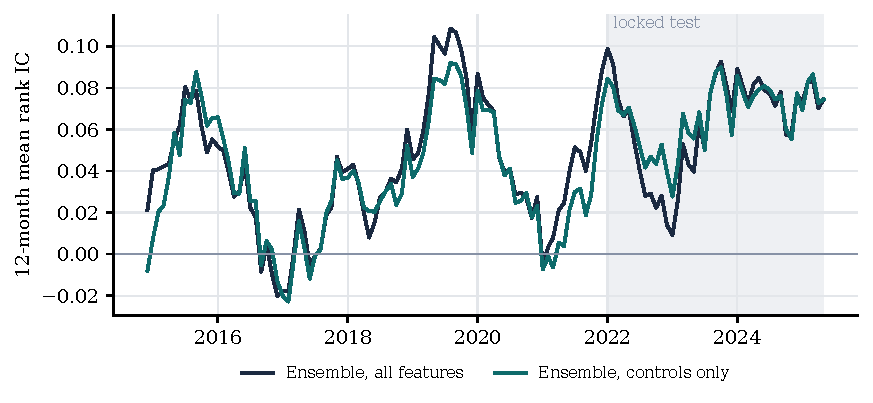
\includegraphics[width=\textwidth]{figures/ic.pdf}
\caption{Twelve-month rolling mean of the monthly rank IC, ensemble with all features against ensemble with controls only.
Shaded: locked test window.}
\label{fig:ic}
\end{figure}

\subsection{The primary strategy}

Figure~\ref{fig:cum} plots the growth of a dollar in the primary strategy and its legs, and Table~\ref{tab:variants}
reports all construction variants. In the development window the primary strategy returns \DevNetMean{} a year net of costs
(Sharpe \DevNetSharpe), with an FF5 + momentum alpha of \DevNetAlpha{} ($t=\DevNetAlphat$). In the locked test it returns
\TestNetMean{} a year net (Sharpe \TestNetSharpe, gross \TestGrossSharpe), but its alpha is \TestNetAlpha{} ($t=\TestNetAlphat$):
the positive raw return is explained by its factor exposures (Table~\ref{tab:alphas}). Turnover is high: buys plus sells in
both legs equal \Turnover{} of one leg's capital a month (about \TurnoverOneWay{} one-way per leg), with \NamesPerLeg{}
stocks per leg, so costs of 25 basis points remove most of the gross return. Figure~\ref{fig:deciles} shows why the
development-window spread is small: decile returns rise with the forecast from the second decile upward, but the bottom
decile also does well. In the test window the bottom decile does poorly, which is where most of the test-window return
comes from.

\begin{figure}[tbp]
\centering
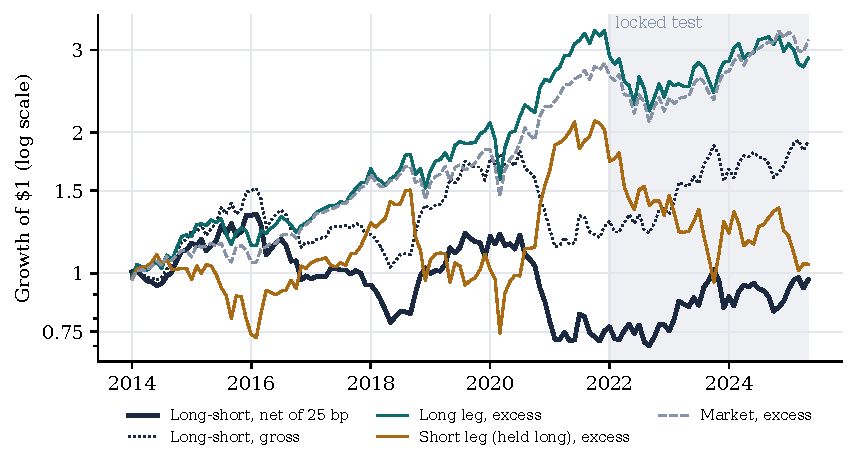
\includegraphics[width=\textwidth]{figures/cum.pdf}
\caption{Growth of \$1 in the primary strategy (ensemble, all features, value-weighted top-minus-bottom decile) from 2014.
The legs are shown as excess returns over T-bills; the short leg is plotted as if held long. Shaded: locked test window.}
\label{fig:cum}
\end{figure}

\begin{figure}[tbp]
\centering
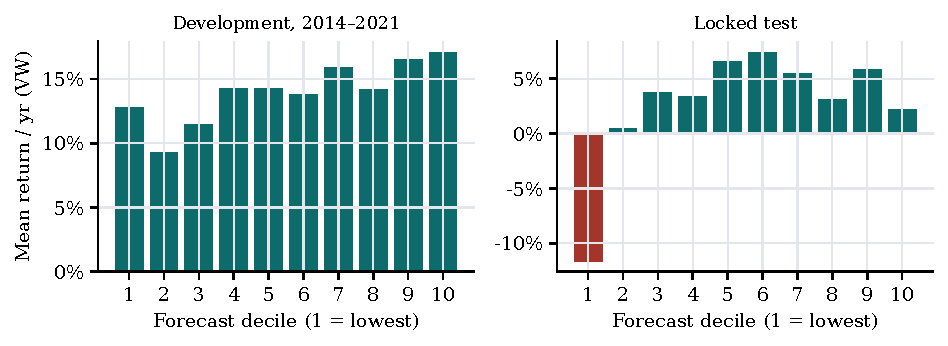
\includegraphics[width=\textwidth]{figures/deciles.pdf}
\caption{Mean annualised return of value-weighted forecast deciles, development and locked test windows.}
\label{fig:deciles}
\end{figure}

\begin{table}[tbp]
\centering
\caption{Strategy construction variants}
\label{tab:variants}
\wide{tab_variants}
\tnote{All variants use the ensemble forecast from all features. Mean, volatility, Sharpe, $t$ and maximum drawdown are gross
of costs. Turnover: buys plus sells in both legs as a share of one leg's capital per month. Net Sharpe and net $t_\alpha$
(FF5 + momentum) after 25 basis points one-way. $t_\alpha$ +LowVol adds a low-minus-high volatility factor built in this
universe. Break-even: the one-way cost that would set the gross mean to zero.}
\end{table}

\begin{table}[tbp]
\centering
\caption{Factor alphas of the primary strategy and its legs}
\label{tab:alphas}
\wide{tab_alphas}
\tnote{Annualised intercepts of time-series regressions, Newey-West(6) $t$-statistics. Long and short legs are excess
returns over T-bills.}
\end{table}

\subsection{Summary of the hypotheses}

\begin{table}[tbp]
\centering
\caption{Hypothesis outcomes}
\label{tab:ledger}
\small
\begin{tabularx}{\textwidth}{@{}llX@{}}
\toprule
 & Verdict & Evidence \\
\midrule
H1 & Partly supported & No level sort earns alpha (largest $|t_\alpha|=\HoneMaxAbsAlphat$), as predicted; but the pre-registered volatility test fails (operations $t=\VolOpst$, aggregate $t=\VolAllt$). Exploratory: \VolSigCount{} of 8 factors predict volatility, \VolUp{} higher and \VolDown{} lower. \\
H2 & Not supported & Most negative of \HtwoN{} statistics $t=\HtwoMinT$. \\
H3 & Below hurdle & Right sign throughout; best $t=\HthreeMaxT$ (\HthreeBest). \\
H4 & Below hurdle & FM interaction $t\leq\HfourFMmax$; double-sort cushion right-signed for risk changes ($t_\alpha\leq\CushionChangeHi$), wrong-signed for levels. \\
H5 & Not supported & Text adds \IncEns{} to the IC ($t=\IncEnst$); primary net alpha $t=\DevNetAlphat$ (development), $\TestNetAlphat$ (test). \\
\bottomrule
\end{tabularx}
\tnote{``Supported'' requires $|t|\geq3$ in the predicted direction; ``below hurdle'' marks a correct sign with $2\leq t<3$, a
descriptive tier that was not pre-registered.}
\end{table}

Table~\ref{tab:ledger} collects the verdicts. No return hypothesis clears the pre-registered hurdle.

%=====================================================================
\section{Robustness and overfitting}\label{sec:robust}
%=====================================================================

\subsection{Is the forecasting skill real?}

The forecasts' predictive content survives every placebo. When the primary forecast is shuffled across stocks within each
month \PlaceboDraws{} times, no shuffled IC comes close to the real one (95th percentile \PlaceboNullICNinetyFive; $p=\PlaceboPic$).
The real gross Sharpe ratio (\PlaceboRealSharpe) lies just above the placebo 95th percentile (\PlaceboNullNinetyFive; $p=\PlaceboPsharpe$;
Figure~\ref{fig:placebo}). Retraining LightGBM on labels shuffled within each month gives an IC of \ShuffledIC{} ($t=\ShuffledICt$),
so the pipeline does not manufacture predictability.

\begin{figure}[tbp]
\centering
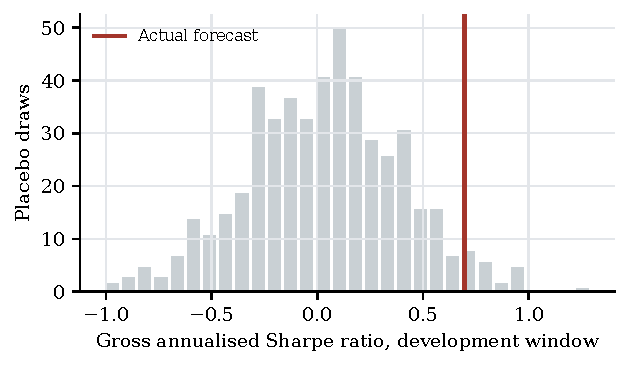
\includegraphics[width=0.62\textwidth]{figures/placebo.pdf}
\caption{Gross Sharpe ratio of the primary portfolio with forecasts shuffled within each month (\PlaceboDraws{} draws) and the
actual value, development window.}
\label{fig:placebo}
\end{figure}

\subsection{Is the strategy real?}

The multiple-testing diagnostics say no (Table~\ref{tab:mt}). Against the \DSRTrials{} logged development specifications,
the deflated Sharpe ratio gives a probability of only \DSR{} that the primary strategy's true Sharpe ratio exceeds the best
one would expect from that many trials by chance (0.95 would be convincing). Across \PBOstrategies{} model and feature-set
combinations and \PBOsplits{} combinatorial splits, the probability that the in-sample winner underperforms the median
out of sample is \PBO{} (below 0.5 is the goal). Model selection on this data mostly picks noise.

\begin{table}[tbp]
\centering
\caption{Multiple-testing and placebo diagnostics}
\label{tab:mt}
\small
\begin{tabular}{lr}
\toprule
Diagnostic & Value \\
\midrule
Development specifications logged (trials) & \DSRTrials \\
Deflated Sharpe probability, primary strategy (gross) & \DSR \\
Probability of backtest overfitting (CSCV, 16 blocks) & \PBO \\
Placebo $p$-value, IC (\PlaceboDraws{} within-month shuffles) & \PlaceboPic \\
Placebo $p$-value, Sharpe ratio & \PlaceboPsharpe \\
Shuffled-label retraining: IC ($t$) & \ShuffledIC{} (\ShuffledICt) \\
IC added by text, ensemble ($t$) & \IncEns{} (\IncEnst) \\
\bottomrule
\end{tabular}
\end{table}

\subsection{Subperiods, size and timing}

The primary strategy's alpha is insignificant in both halves of the development window ($t_\alpha=\SubAt$ in 2014--2017 and
\SubBt{} in 2018--2021) and it lost \CovidMean{} (annualised) in 2020 (Table~\ref{tab:sub}). Predictability is concentrated in
small stocks (mean IC \SmallIC{} against \MidIC{} and \LargeIC{} for mid and large stocks; Table~\ref{tab:size}), where trading
costs are highest. Changing the release lags of either text source, adding or removing the call-coverage flag, using the
raw rather than whitened marketing components, or forecasting three-month returns leaves the IC essentially unchanged
(Table~\ref{tab:altspec}). In the extended equal-weighted sample from 2006, which adds the financial crisis but has no size
data, the aggregate-risk long-short earns \ExtRiskAllMean{} a year (Sharpe \ExtRiskAllSharpe, $t=\ExtRiskAllt$), again
positive and again below the hurdle (Table~\ref{tab:ext}).

\begin{table}[tbp]
\centering
\caption{Subperiods, primary strategy net of costs}
\label{tab:sub}
\small
\begin{tabular}{lrrrrrr}
\toprule
Period & Months & Net mean / yr & Sharpe & $t$ & $\alpha$ / yr & $t_\alpha$ \\
\midrule
2014-2017 & 48 & \ensuremath{-}0.4\% & \ensuremath{-}0.03 & \ensuremath{-}0.06 & \ensuremath{-}3.2\% & \ensuremath{-}0.72 \\
2018-2021 & 48 & \ensuremath{-}3.8\% & \ensuremath{-}0.20 & \ensuremath{-}0.32 & \ensuremath{-}4.4\% & \ensuremath{-}0.58 \\
2020 (COVID) & 12 & \ensuremath{-}19.4\% & \ensuremath{-}0.87 & \ensuremath{-}0.87 & -- & -- \\
Test, 2022-01--2025-05 & 41 & 8.9\% & 0.51 & 1.46 & \ensuremath{-}4.6\% & \ensuremath{-}0.83 \\
\bottomrule
\end{tabular}

\tnote{FF5 + momentum alpha omitted for the 12-month 2020 window.}
\bigskip
\caption{Predictability by size tercile}
\label{tab:size}
\begin{tabular}{lrrrrr}
\toprule
Size tercile & Names / mo & Mean IC & EW Q5$-$Q1 / yr & Sharpe & $t$ \\
\midrule
Small & 386 & 0.051 & 12.7\% & 0.97 & \textbf{3.02} \\
Mid & 386 & 0.026 & 3.5\% & 0.29 & 0.80 \\
Large & 387 & 0.028 & 6.9\% & 0.69 & 1.72 \\
\bottomrule
\end{tabular}

\tnote{Development window, ensemble forecast, equal-weighted top-minus-bottom quintile within each size tercile, gross.}
\end{table}

\begin{table}[tbp]
\centering
\caption{Alternative timing, features and horizon (LightGBM unless stated)}
\label{tab:altspec}
\small
\begin{tabular}{lrrr}
\toprule
Specification (development OOS, 2014--2021) & Rank IC & $t$ & Hit rate \\
\midrule
\multicolumn{4}{l}{\textit{Panel A: timing variants}} \\
Baseline (LightGBM, all features) & 0.0409 & \textbf{3.79} & 51.6\% \\
Call scores one month earlier (no buffer) & 0.0428 & \textbf{4.32} & 51.6\% \\
Call scores one month later & 0.0400 & \textbf{3.78} & 51.3\% \\
10-K scores 10 business days after filing & 0.0412 & \textbf{3.63} & 51.5\% \\
\midrule
\multicolumn{4}{l}{\textit{Panel B: feature diagnostics}} \\
Controls + call-coverage flag & 0.0351 & \textbf{3.41} & 51.2\% \\
Controls + marketing, no flag & 0.0425 & \textbf{4.13} & 51.5\% \\
Controls + marketing & 0.0423 & \textbf{3.98} & 51.5\% \\
Controls + risk + raw marketing components & 0.0429 & \textbf{4.00} & 51.5\% \\
\midrule
\multicolumn{4}{l}{\textit{Panel C: horizon}} \\
3-month target: + interactions (all), Elastic net & 0.0379 & 1.89 & 51.5\% \\
3-month target: Controls only, LightGBM & 0.0430 & 2.25 & 51.4\% \\
3-month target: + interactions (all), LightGBM & 0.0493 & 2.67 & 51.7\% \\
\bottomrule
\end{tabular}

\tnote{Development out-of-sample window. Timing variants rebuild the whole panel under the alternative lag.}
\end{table}

\begin{table}[tbp]
\centering
\caption{Extended equal-weighted sample including 2008--2009}
\label{tab:ext}
\small
\begin{tabular}{lrrrrr}
\toprule
Signal (EW decile L/S, 2006--2021) & Months & Mean / yr & Sharpe & $t$ & Max DD \\
\midrule
Non-operational risk (7 factors) & 186 & 4.5\% & 0.81 & 2.73 & \ensuremath{-}14\% \\
Aggregate risk (8 factors) & 186 & 6.1\% & 0.82 & 2.67 & \ensuremath{-}25\% \\
Operations risk & 186 & 4.8\% & 0.43 & 1.63 & \ensuremath{-}23\% \\
$\Delta$ operations risk & 177 & \ensuremath{-}1.9\% & \ensuremath{-}0.37 & \ensuremath{-}1.42 & \ensuremath{-}30\% \\
\bottomrule
\end{tabular}

\tnote{Equal-weighted decile long-short portfolios from 2006-07; no size filter or value weights are possible before XBRL.}
\end{table}

\subsection{What the model uses}

SHAP values \citep{lundberg2017} for the LightGBM model trained for the first test year (Figure~\ref{fig:shap}) show
that one-month reversal is the single most important feature. By group, marketing features account for \ShapMkt{} of mean
absolute SHAP, controls \ShapCtrl, risk text \ShapRisk{} and interactions \ShapInter. Part of the marketing block's value
is simply whether a firm has scored calls at all, which proxies for size and analyst attention. The coverage-flag
diagnostic in Table~\ref{tab:altspec} separates the two: for LightGBM, the IC rises from \DiagC{} with controls to \DiagFlag{}
with the flag alone and \DiagCM{} with the marketing scores, so the flag accounts for about \DiagFlagShare{} of the gain and the
scores themselves for the rest. That gain is real but small, and it does not reach a tradable alpha.

\begin{figure}[tbp]
\centering
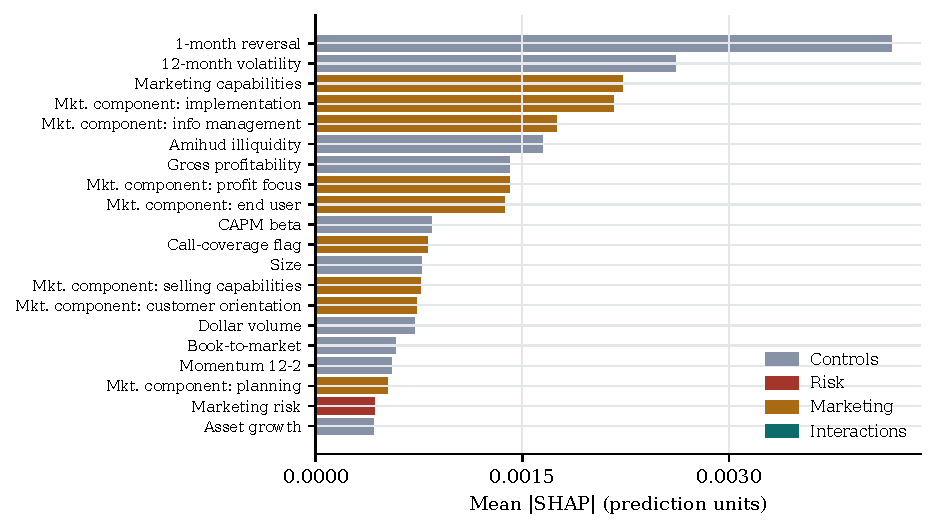
\includegraphics[width=0.75\textwidth]{figures/shap.pdf}
\caption{Twenty most important features by mean absolute SHAP value, LightGBM with all features trained through 2021-11
(\ShapLeaves{} leaves, \ShapTrees{} trees). Colour: feature group.}
\label{fig:shap}
\end{figure}

%=====================================================================
\section{Further evidence}\label{sec:further}
%=====================================================================

Three supplementary studies were added after the design was frozen. They test the data rather than a trading rule and are
not counted as strategy trials.

\subsection{A survivorship audit}\label{sec:surv}

Free price data covers only firms that still trade, so firms that went bankrupt, were acquired or were delisted are missing,
and more so in early years. CRSP with delisting returns \citep{shumway1997} is the standard remedy, but it was not available.
The SEC, however, keeps the complete filing history of every registrant, including those that disappeared. For each
non-empty 10-K of a non-financial, non-utility firm that ever had CRSP-listed stock (proxied by a CRSP/Compustat link in the
WRDS table), we record whether we observe its price within twelve months of the filing and how the firm ended: still filing
in 2025 or later; bankrupt (an 8-K under item 1.03 within three years before its last filing); acquired (merger proxy or
tender-offer forms within two years before its last filing); or another exit.

Of \FateTotal{} such firms, \FateSurv{} still file, \FateMerged{} were acquired, \FateBankrupt{} went bankrupt and \FateOther{} left
for other reasons. Our prices cover \CovTwoThousandSix{} of their 2006 filings and \CovTwentyTwentyFour{} of their 2024 filings
(Figure~\ref{fig:surv}, Table~\ref{tab:survcov}). Among missing firms, acquisitions far outnumber bankruptcies.

The key question is whether the bias favours high-risk stocks. It does not. Among 2010--2021 filings, \MissLowRisk{} of the
lowest decile of aggregate risk is missing against \MissHighRisk{} of the highest (Table~\ref{tab:survbe}). If the missing firms
were restored to their deciles, the observed value-weighted high-minus-low spread would vanish only if they had outperformed
the observed firms in their decile by \BreakevenVW{} a month (\BreakevenEW{} equal-weighted). That is implausible for a group that
includes every bankruptcy. Survivorship therefore cannot have produced the positive risk spread; if anything it understates
it. The audit cannot score the machine-learning strategy's short leg, which would need forecasts for firms without prices.

\begin{figure}[tbp]
\centering
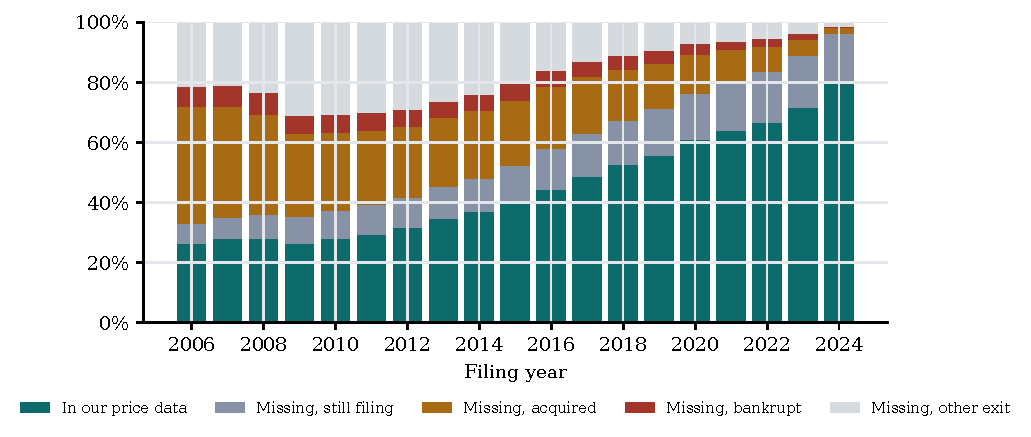
\includegraphics[width=\textwidth]{figures/survivorship.pdf}
\caption{Share of once-listed 10-K filers in our price data, by filing year and eventual fate.}
\label{fig:surv}
\end{figure}

\begin{table}[tbp]
\centering
\caption{Survivorship audit: coverage of once-listed filers}
\label{tab:survcov}
\small
\begin{tabular}{lrrrrrr}
\toprule
Filing year & Filings & Covered & Still filing & Acquired & Bankrupt & Other exit \\
\midrule
2007 & 3{,}849 & 28\% & 7\% & 37\% & 7\% & 21\% \\
2010 & 4{,}942 & 28\% & 9\% & 26\% & 6\% & 31\% \\
2013 & 4{,}570 & 35\% & 11\% & 23\% & 6\% & 26\% \\
2016 & 4{,}193 & 44\% & 13\% & 21\% & 5\% & 16\% \\
2019 & 3{,}917 & 56\% & 16\% & 15\% & 4\% & 9\% \\
2022 & 4{,}388 & 67\% & 17\% & 8\% & 3\% & 5\% \\
\bottomrule
\end{tabular}

\tnote{Shares of each year's filings. ``Covered'': a monthly price is observed within twelve months after the filing.
The remaining columns split the uncovered filings by the firm's fate.}
\end{table}

\begin{table}[tbp]
\centering
\caption{Survivorship audit: missing firms by risk decile and break-even return gap}
\label{tab:survbe}
\wide{tab_survbe}
\tnote{Observed L/S: development-window decile spread from Table~\ref{tab:single}. Missing shares: 2010--2021 filings of
once-listed firms absent from our price data, in the top and bottom within-year decile of the signal. Break-even gap $g^*$
solves $\text{spread} + (m_{\text{top}}-m_{\text{bottom}})\,g^* = 0$: the monthly return by which missing firms would have to
beat observed firms in the same decile for the spread to vanish.}
\end{table}

As a by-product, the audit tests whether risk language anticipates how firms end (Table~\ref{tab:survlpm}), on a sample that
includes the firms missing from our prices. Moving from the lowest to the highest rank of finance-risk language adds
\BkFinancePP{} percentage points to the probability of bankruptcy within three years ($t=\BkFinancet$; base rate \BkBase), and
operations risk adds \BkOpsPP{} points ($t=\BkOpst$). Technology, marketing and international risk language instead predict
acquisition (technology $t=\MgTecht$; base rate \MgBase). This is direct evidence that the transformer scores capture real
differences in firm risk.

\begin{table}[tbp]
\centering
\caption{Does risk language predict how a firm ends? (filings 2006--2022)}
\label{tab:survlpm}
\small
\begin{tabular}{lrrrrrr}
\toprule
Risk measure & Bankruptcy (pp) & $t$ & Acquisition (pp) & $t$ & Any exit (pp) & $t$ \\
\midrule
Aggregate risk (8 factors) & 0.7 & 1.43 & 11.3 & \textbf{12.62} & 4.4 & \textbf{3.59} \\
Non-operational risk & 0.3 & 0.98 & 2.7 & \textbf{5.37} & 1.2 & 1.95 \\
Accounting risk & \ensuremath{-}0.5 & \ensuremath{-}1.57 & \ensuremath{-}0.9 & \ensuremath{-}1.86 & \ensuremath{-}0.8 & \ensuremath{-}1.20 \\
Finance risk & 3.0 & \textbf{8.59} & \ensuremath{-}1.6 & \textbf{\ensuremath{-}3.10} & \ensuremath{-}0.8 & \ensuremath{-}1.24 \\
International risk & \ensuremath{-}1.0 & \textbf{\ensuremath{-}3.28} & 4.1 & \textbf{8.35} & \ensuremath{-}0.9 & \ensuremath{-}1.35 \\
Legal risk & 0.8 & 2.52 & 4.7 & \textbf{9.10} & 4.4 & \textbf{6.77} \\
Management risk & \ensuremath{-}0.2 & \ensuremath{-}0.66 & 3.5 & \textbf{7.46} & 2.5 & \textbf{4.14} \\
Marketing risk & \ensuremath{-}0.7 & \ensuremath{-}2.35 & 5.0 & \textbf{9.82} & 1.7 & 2.69 \\
Operations risk & 1.5 & \textbf{4.64} & 2.0 & \textbf{3.92} & 0.3 & 0.46 \\
Technology risk & \ensuremath{-}1.3 & \textbf{\ensuremath{-}4.31} & 7.4 & \textbf{14.26} & 2.8 & \textbf{4.24} \\
\bottomrule
\end{tabular}

\tnote{Linear probability models of each outcome within 36 months of the 10-K on the within-year rank of one risk measure
(coefficient = change from lowest to highest rank, in percentage points), with filing-year fixed effects and
firm-clustered $t$-statistics \citep{petersen2009}. $N=\BkN$ filings, including firms absent from our price data.}
\end{table}

\subsection{The market's reaction on filing day}

If investors read the risk sections, prices should react when the 10-K appears; if they underreact, returns should drift
afterwards. For \EvN{} 10-Ks of \EvFirms{} firms in the primary universe (2010--2024), we compute market-adjusted returns from
the filing day to the next ($[0,+1]$), its absolute value, the drift over days $+2$ to $+60$, and the change in the
volatility of daily abnormal returns from the year before to the quarter after the filing. Each is regressed, year by year,
on a point-in-time risk rank and the ten controls (Table~\ref{tab:event}). Legal-risk language comes with larger filing-day
moves ($t=\EvLegalAbst$), while most other risk types go with smaller ones. No risk measure predicts the post-filing drift
(all $|t|\leq\EvDriftMaxAbst$). Investors respond to some risk content at the filing, but leave no exploitable drift, which
is consistent with the null result for risk changes (H2).

\begin{table}[tbp]
\centering
\caption{Filing-date event study, 2010--2024}
\label{tab:event}
\wide{tab_event}
\tnote{Fama-MacBeth slopes across filing years of each outcome on the risk rank (lowest to highest = 1), with the ten
controls. CAR: cumulative market-adjusted return (daily Mkt-RF + RF), winsorised at 1\%/99\% within year.
$\Delta\ln\sigma$: log ratio of the standard deviation of daily abnormal returns over days $[+2,+61]$ to that over
$[-250,-21]$. Signals are the panel's ranks in the filing's first usable month; controls are measured before the filing.}
\end{table}

\subsection{Replicating the source paper}

\citet{astvansh2026} report that operational risk in year $y$ predicts higher log cost of goods sold (COGS) in $y+1$, with
firm and year fixed effects (their Table~7). We rebuild the regression from SEC XBRL instead of Compustat: \RepN{} firm-years
of \RepFirms{} firms, fiscal years \RepYearLo--\RepYearHi, including firms that later disappeared. Year $y$ is the fiscal year
reported in each 10-K, and the controls follow their definitions (log total assets, the optional-Item-1A flag, log section
length and R\&D over assets). Table~\ref{tab:rep} shows that the main effect replicates in size: \RepOpFour{} (SE \RepOpFourSE)
against their 0.247 (0.041), and \RepOpTwo{} against their 0.222 without the non-operational terms. Our standard errors are
wider, on roughly half their sample. Their positive interaction between operational and non-operational risk does not
replicate ($t=\RepIntert$). We also note two inconsistencies in their variable definitions: firm size is described as log
revenue in the text but log assets in their Table~5, and R\&D as a share of revenue in the text but of assets in the formula.
We follow their Table~5.

\begin{table}[tbp]
\centering
\caption{Replication of Astvansh and Simpson (2026), Table 7}
\label{tab:rep}
\small
\begin{tabular}{lrrrr}
\toprule
 & This study (2) & Paper (2) & This study (4) & Paper (4) \\
\midrule
Operational risk & 0.275 (0.100) & 0.222 (0.038) & 0.289 (0.107) & 0.247 (0.041) \\
Non-operational risk &  &  & \ensuremath{-}0.009 (0.067) & \ensuremath{-}0.046 (0.024) \\
Operational $\times$ non-operational &  &  & 0.149 (0.398) & 0.298 (0.125) \\
$\ln$(total assets)$_{y}$ & 0.415 (0.022) & 0.486 (0.014) & 0.415 (0.022) & 0.486 (0.014) \\
Item 1A optional & 0.014 (0.060) & \ensuremath{-}0.093 (0.025) & 0.017 (0.060) & \ensuremath{-}0.083 (0.025) \\
$\ln$(Item 1A words) & \ensuremath{-}0.004 (0.012) & \ensuremath{-}0.007 (0.003) & \ensuremath{-}0.002 (0.016) & 0.001 (0.004) \\
R\&D / assets & 0.064 (0.143) & 0.004 (0.014) & 0.064 (0.143) & 0.004 (0.014) \\
Firm-years & 34{,}960 & 67{,}727 & 34{,}960 & 67{,}727 \\
Firm and fiscal-year FE & Yes & Yes & Yes & Yes \\
\bottomrule
\end{tabular}

\tnote{Dependent variable: $\ln$(COGS) in fiscal year $y+1$, winsorised at 1\%/99\%. Operational and non-operational risk are
mean-centred probabilities (non-operational = sum of the seven other types). Standard errors clustered by firm in
parentheses. Columns (2) and (4) follow their Table~7.}
\end{table}

%=====================================================================
\section{Discussion}\label{sec:discussion}
%=====================================================================

The evidence points to one consistent picture: the risk scores are informative about \emph{risk}, not about
\emph{mispricing}. They predict how volatile a stock will be, whether the firm will fail, and how strongly the market moves
when the filing appears, and they relate to future costs as their authors found. But none of this information earns an
abnormal return once standard characteristics and factors are accounted for, and the market does not drift after filings.
This is what an efficient market would produce for public, slowly changing, widely read disclosures. The small positive
spread on aggregate risk language is the sign of a modest risk premium rather than of an anomaly, and our survivorship
audit suggests that it is understated rather than overstated by the free data. The link from these risk categories to
returns documented by \citet{schnatterly2021} runs through whether the board has the expertise to manage the disclosed
risks. Our results are consistent with that view: the disclosure on its own, without information on who governs the
risks, does not forecast returns.

Why does the text add so little to the forecasts? Three reasons stand out. First, the scores change slowly: a 10-K arrives
once a year and a firm's probabilities are persistent from one filing to the next, so much of their cross-sectional
content is about stable firm types already captured by size, volatility and industry. Second, the probabilities measure the
\emph{share} of risk language rather than its amount, and the scores relate only loosely to their own dictionary counts,
which adds measurement noise. Third, the controls that dominate return forecasts at a monthly horizon, such as short-term
reversal and volatility, are price-based and fast-moving; annual text cannot compete with them at that horizon.

The marketing scores are a partial exception. Their returns have the predicted sign throughout and come closest to the
hurdle, and the marketing block is the largest in the SHAP decomposition. But its gain over the controls is small, about
\DiagFlagShare{} of it comes from whether a firm has scored calls at all, which proxies for size and analyst coverage, and
the constructs are nearly collinear. A cleaner test would need call dates, transcripts and a longer sample.

Two methodological lessons are worth recording. The first is the value of a locked test window. Our first test-window run
produced a Sharpe ratio above 1.5 and alphas with $t$-statistics up to 5. The locked window made that result suspicious
enough to investigate, and the cause was a look-ahead in the free price data (Appendix~\ref{app:bug}). Without the lock, the
result would have been folded into the development window and might never have been questioned. The second is that the
multiple-testing diagnostics agreed with the economics: a deflated Sharpe probability of \DSR{} and a probability of
overfitting of \PBO{} say the same as the factor alphas, from a different direction.

%=====================================================================
\section{Limitations}\label{sec:limits}
%=====================================================================

\begin{itemize}
  \item \textbf{Survivorship.} Prices exist only for firms that still traded in November 2026, so a 2014 stock had to survive
  about twelve more years and a 2023 stock about three. The audit in Section~\ref{sec:surv} bounds the effect on the risk
  sorts but cannot score the machine-learning strategy's short leg. Development and test results are not directly comparable.
  \item \textbf{Free fundamentals and identifiers.} Size and book data come from XBRL and start in 2009--2011; industry codes,
  tickers and exchanges are today's, applied backwards.
  \item \textbf{Score validity.} The risk transformers were trained on synthetic sentences labelled by dictionaries, with no
  human-labelled validation on real filings. The marketing constructs are near-collinear, and the authors' whitening was
  probably estimated on the full 2003--2025 sample, a mild look-ahead that a robustness run with raw components addresses.
  \item \textbf{No call dates.} Marketing scores are dated by calendar quarter, which forces a conservative lag.
  \item \textbf{Short test window.} \TestMonths{} months cannot by themselves separate a modest edge from luck; the test is a check
  on the development results, not a verdict on its own.
  \item \textbf{Costs.} We charge commissions and spread through a flat one-way cost but not market impact or short-borrowing fees,
  which would make the strategy look worse.
\end{itemize}

%=====================================================================
\section{Conclusion}\label{sec:conclusion}
%=====================================================================

Under strict point-in-time rules, a locked test window and an honest count of the specifications we tried, transformer
scores of 10-K risk disclosures and embedding scores of earnings-call marketing language do not provide a profitable
long-short strategy and add little to the return forecasts of standard characteristics. They do measure real differences
in firm risk: they predict volatility, bankruptcy and filing-day price moves, and they reproduce their source paper's
link to future operating costs. For researchers, the scores are better suited to studying risk and firm outcomes than to
forecasting returns. For practitioners, the result is a reminder that informative text is not the same as profitable text.
Natural extensions are a survivorship-free price source, the same transformers applied to quarterly 10-Q risk updates,
call-level timing for the marketing scores, and director expertise from proxy statements. The last would test, in the
spirit of \citet{schnatterly2021}, whether the transformer risk scores predict returns for firms whose boards lack
expertise in the risks they disclose.

\bibliographystyle{plainnat}
\bibliography{references}

\appendix

%=====================================================================
\section{Data audit highlights}\label{app:audit}
%=====================================================================

\begin{itemize}
  \item \textbf{Fiscal year.} \texttt{FYEAR} equals the calendar year of \texttt{Filing Date} in every row of the risk data.
  Amazon's \texttt{FYEAR}~2024 row is its fiscal-2023 10-K filed in February 2024. A ``January--June means previous year''
  heuristic, used in an earlier version of this project, misassigns most December year-end filers.
  \item \textbf{Filing dates.} Joining on CIK and filing date to EDGAR's quarterly form indices matches an original 10-K for
  every filing except the three filed in January 2025, which fall outside the cached indices.
  \item \textbf{Empty sections.} 9,320 filings have zero Item 1A words and all-zero probabilities; they are treated as missing.
  \item \textbf{Score means.} The mean probabilities match Table~4 of \citet{astvansh2026} to three decimals, confirming that we
  hold the same release.
  \item \textbf{Marketing file.} The executive file has no duplicate (GVKEY, year, quarter) keys and no missing values; 1,158
  rows of the 2023--2025 extension carry several GVKEYs in one cell and are split before linking. An earlier version of this
  project averaged only 11 of the 19 components into the three constructs; we use all 19.
  \item \textbf{Links.} 85\% of risk CIKs appear in the WRDS link table; about 5,000 firms have both risk and marketing scores.
\end{itemize}

%=====================================================================
\section{A look-ahead bug caught by the locked test window}\label{app:bug}
%=====================================================================

The first run of the locked test window produced value-weighted Sharpe ratios of 1.5 to 2.0 and FF5 + momentum alphas with
$t$-statistics up to 5.3, far above the development-window results. Rather than accept the result, we traced the
strategy's best months to individual stocks. The cause was in the price download. Yahoo Finance's split-adjusted close
reflects every split up to the download date, but the price request had been capped at the end of 2025, so splits executed
in 2026 were missing from the split events we used to adjust share counts. For firms with large reverse splits in 2026
(for example, ratios of 1:25 and 1:3,000), prices were already adjusted while shares were not, which made their historical
market capitalisations, and hence size screens and value weights, depend on events that had not yet happened.

We removed the end date from the download, rebuilt every derived file, and archived the affected results under a
\texttt{BUGGY} label. After the fix, the test-window strategy no longer earns a significant alpha. A unit test now asserts
that the price download has no end date. We report the episode because it shows how free price data can leak the future
through split adjustments, and because the locked window is what made the leak visible.

%=====================================================================
\section{Selected design decisions}\label{app:decisions}
%=====================================================================

The project's decision log records every methodological choice, with alternatives and reasons. The most consequential are:
\begin{itemize}
  \item \textbf{Market capitalisation from free data.} Close price times split-adjusted XBRL shares; share counts that jump more
  than tenfold against the median of the three previous values are discarded, as are capitalisations above \$5 trillion,
  turnover outside 0.1\% to 500\% a month, and capitalisations above 500 times book assets.
  \item \textbf{Capped value weights.} Capitalisation winsorised each month at the 80th percentile of NYSE-listed stocks in the
  universe \citep{jkp2023}.
  \item \textbf{Return cleaning.} Only impossible returns are removed; a rule that used the next month's return to judge the
  current one was dropped because it looked ahead.
  \item \textbf{Ensemble.} Averages within-month ranks of the four learners, as pre-registered. Averaging raw predictions,
  as an early version did, lets the learner with the widest prediction spread dominate.
  \item \textbf{Trial family for the deflated Sharpe ratio.} Every development-window specification in the log, including
  construction variants of the primary strategy and the double sorts added for H4; test-window runs are excluded.
  \item \textbf{Sample end.} 2025-05: in 2025-06 the universe halves because 10-Ks filed after January 2025 are not in the risk data.
  \item \textbf{Independent reviews.} Two independent code and documentation reviews were run before the final results; their
  findings (the rank ensemble, the sample end, the horizon-3 embargo, the cleaning rule, the trial family and several prose
  corrections) are applied and logged.
\end{itemize}

%=====================================================================
\section{Reproducibility}\label{app:repro}
%=====================================================================

All results come from one command, \texttt{python run\_all.py}, which runs the stages download, panel, features, tests,
single-signal tests, machine learning, analysis, supplementary studies, export, notebooks and this report. Downloads are
frozen after the first run. Every result in this report (each estimate, statistic, table and figure) is generated from
the pipeline's outputs by \texttt{report/make\_report\_assets.py}; the only numbers typed by hand are design parameters,
counts from the data audit and values quoted from the cited papers. The test suite checks the timing rules on the final panel,
the walk-forward embargo, portfolio arithmetic, the event-study windows and the survivorship classification. The code,
the data audit and the decision log are in the project repository,
\url{https://github.com/Yugdes/Long-Short-Equity-Strategy-from-10-K-Earnings-Call-NLP-Signals}. An interactive website
presenting the results, rebuilt automatically from the same outputs, is at
\url{https://yugdes.github.io/Long-Short-Equity-Strategy-from-10-K-Earnings-Call-NLP-Signals/}.

\end{document}
